% Options for packages loaded elsewhere
\PassOptionsToPackage{unicode}{hyperref}
\PassOptionsToPackage{hyphens}{url}
%
\documentclass[
  12pt,
]{article}
\usepackage{lmodern}
\usepackage{amsmath}
\usepackage{ifxetex,ifluatex}
\ifnum 0\ifxetex 1\fi\ifluatex 1\fi=0 % if pdftex
  \usepackage[T1]{fontenc}
  \usepackage[utf8]{inputenc}
  \usepackage{textcomp} % provide euro and other symbols
  \usepackage{amssymb}
\else % if luatex or xetex
  \usepackage{unicode-math}
  \defaultfontfeatures{Scale=MatchLowercase}
  \defaultfontfeatures[\rmfamily]{Ligatures=TeX,Scale=1}
  \setmainfont[]{Times New Roman}
\fi
% Use upquote if available, for straight quotes in verbatim environments
\IfFileExists{upquote.sty}{\usepackage{upquote}}{}
\IfFileExists{microtype.sty}{% use microtype if available
  \usepackage[]{microtype}
  \UseMicrotypeSet[protrusion]{basicmath} % disable protrusion for tt fonts
}{}
\makeatletter
\@ifundefined{KOMAClassName}{% if non-KOMA class
  \IfFileExists{parskip.sty}{%
    \usepackage{parskip}
  }{% else
    \setlength{\parindent}{0pt}
    \setlength{\parskip}{6pt plus 2pt minus 1pt}}
}{% if KOMA class
  \KOMAoptions{parskip=half}}
\makeatother
\usepackage{xcolor}
\IfFileExists{xurl.sty}{\usepackage{xurl}}{} % add URL line breaks if available
\IfFileExists{bookmark.sty}{\usepackage{bookmark}}{\usepackage{hyperref}}
\hypersetup{
  pdftitle={What's the Catch? Recreational Fishing Trends in North Carolina (1990-2019)},
  pdfauthor={Ardath Dixon, Annie Harshbarger, Eva May},
  hidelinks,
  pdfcreator={LaTeX via pandoc}}
\urlstyle{same} % disable monospaced font for URLs
\usepackage[margin=2.54cm]{geometry}
\usepackage{graphicx}
\makeatletter
\def\maxwidth{\ifdim\Gin@nat@width>\linewidth\linewidth\else\Gin@nat@width\fi}
\def\maxheight{\ifdim\Gin@nat@height>\textheight\textheight\else\Gin@nat@height\fi}
\makeatother
% Scale images if necessary, so that they will not overflow the page
% margins by default, and it is still possible to overwrite the defaults
% using explicit options in \includegraphics[width, height, ...]{}
\setkeys{Gin}{width=\maxwidth,height=\maxheight,keepaspectratio}
% Set default figure placement to htbp
\makeatletter
\def\fps@figure{htbp}
\makeatother
\setlength{\emergencystretch}{3em} % prevent overfull lines
\providecommand{\tightlist}{%
  \setlength{\itemsep}{0pt}\setlength{\parskip}{0pt}}
\setcounter{secnumdepth}{5}
\usepackage{booktabs}
\usepackage{longtable}
\usepackage{array}
\usepackage{multirow}
\usepackage{wrapfig}
\usepackage{float}
\usepackage{colortbl}
\usepackage{pdflscape}
\usepackage{tabu}
\usepackage{threeparttable}
\usepackage{threeparttablex}
\usepackage[normalem]{ulem}
\usepackage{makecell}
\usepackage{xcolor}
\ifluatex
  \usepackage{selnolig}  % disable illegal ligatures
\fi

\title{What's the Catch? Recreational Fishing Trends in North Carolina
(1990-2019)}
\usepackage{etoolbox}
\makeatletter
\providecommand{\subtitle}[1]{% add subtitle to \maketitle
  \apptocmd{\@title}{\par {\large #1 \par}}{}{}
}
\makeatother
\subtitle{\url{https://github.com/ardathdixon/Data_FinalProject}}
\author{Ardath Dixon, Annie Harshbarger, Eva May}
\date{Spring 2021}

\begin{document}
\maketitle

\newpage
\tableofcontents 
\newpage
\listoftables 
\newpage
\listoffigures 
\newpage

\hypertarget{rationale-and-research-questions}{%
\section{Rationale and Research
Questions}\label{rationale-and-research-questions}}

\begin{itemize}
\item
  Are there trends in the amount of these fish caught over time? How do
  they compare?
\item
  What could these trends look like in the future?
\end{itemize}

\begin{quote}
\emph{Write 1-2 paragraph(s) detailing the rationale for your study.
This should include both the context of the topic as well as a rationale
for your choice of dataset (reason for location, variables, etc.). You
may choose to include citations if you like (optional).}
\end{quote}

\begin{quote}
\emph{At the end of your rationale, introduce a numbered list of your
questions (or an overarching question and sub-questions).}
\end{quote}

\newpage

\hypertarget{dataset-information}{%
\section{Dataset Information}\label{dataset-information}}

Data retrieved from NOAA Marine Recreational Information Program
download query tool

\begin{itemize}
\item
  Bimonthly recreational fisheries catch totals for NC, 1990-2019
\item
  All species, bluefish (\emph{Pomatomus saltatrix}), and black sea bass
  (\emph{Centropristis striata})
\item
  Multiple areas and modes of fishing
\end{itemize}

\begin{quote}
\emph{Provide information on how the dataset for this analysis were
collected, the data contained in the dataset, and any important pieces
of information that are relevant to your analyses. This section should
contain much of same information as the metadata file for the dataset
but formatted in a way that is more narrative.}
\end{quote}

\begin{quote}
\emph{Describe how you wrangled your dataset in a format similar to a
methods section of a journal article.}
\end{quote}

\begin{quote}
\emph{Add a table that summarizes your data structure (variables, units,
ranges and/or central tendencies, data source if multiple are used,
etc.). This table can be made in markdown text or inserted as a
\texttt{kable} function in an R chunk. If the latter, do not include the
code used to generate your table.}
\end{quote}

\begin{table}[H]

\caption{\label{tab:table1}General Information About the Data Used}
\centering
\begin{tabular}[t]{l|l}
\hline
Detail & Description\\
\hline
Data Source & NOAA MRIP\\
\hline
Retrieved from & https://www.fisheries.noaa.gov/data-tools/recreational-fisheries-statistics-queries\\
\hline
Variables Used & Year, Wave, Total Catch, Mode, Area\\
\hline
Date Range & January 1990 - December 2019\\
\hline
\end{tabular}
\end{table}

\begin{table}[H]

\caption{\label{tab:table2}Total Catch Summaries}
\centering
\begin{tabular}[t]{l|r|r|r}
\hline
Summary Statistics & All Fish & Bluefish & Black Sea Bass\\
\hline
Minimum & 11869 & 26 & 1168\\
\hline
Mean & 12402954 & 1342064 & 411196\\
\hline
Median & 11292146 & 1064369 & 313437\\
\hline
Maximum & 34932698 & 5254124 & 1746847\\
\hline
\end{tabular}
\end{table}
\newpage

\hypertarget{exploratory-analysis}{%
\section{Exploratory Analysis}\label{exploratory-analysis}}

We began our analysis by converting waves to months, in order to process
the six annual waves using time series analyses. For NOAA fishing
records, wave 1 represents January and February, wave 2 represents March
and April, and this continues through the year. Therefore, we assigned
wave 1 catches to the date of January 1, wave 2 catches to March 1, and
beyond. We checked the number of waves without catch records for each
dataset by joining the existing data to a list of all possible waves
between Wave 1 of 1990 (represented by 1990-01-01) and Wave 6 of 2019
(2019-11-01). The results of this exploration, which informed our
approach for interpolation, can be found in Table 3.

\begin{table}[H]

\caption{\label{tab:table3}Number of missing values from NOAA MRIP data}
\centering
\begin{tabular}[t]{l|r}
\hline
Dataset & Number of missing values\\
\hline
All fish & 11\\
\hline
Bluefish & 17\\
\hline
Black sea bass & 13\\
\hline
\end{tabular}
\end{table}

To fill the gaps with no data, we interpolated the likely values of
missing time periods. This interpolation incorporated the catch numbers
on either side chronologically. We graphed the total catch trends over
time (with the newly interpolated values for missing periods) as shown
in Figure 1. With this visualization, we could compare the three
categories' recreational fishing catch patterns: all fish, bluefish, and
black sea bass.

\begin{figure}[H]

\hfill{}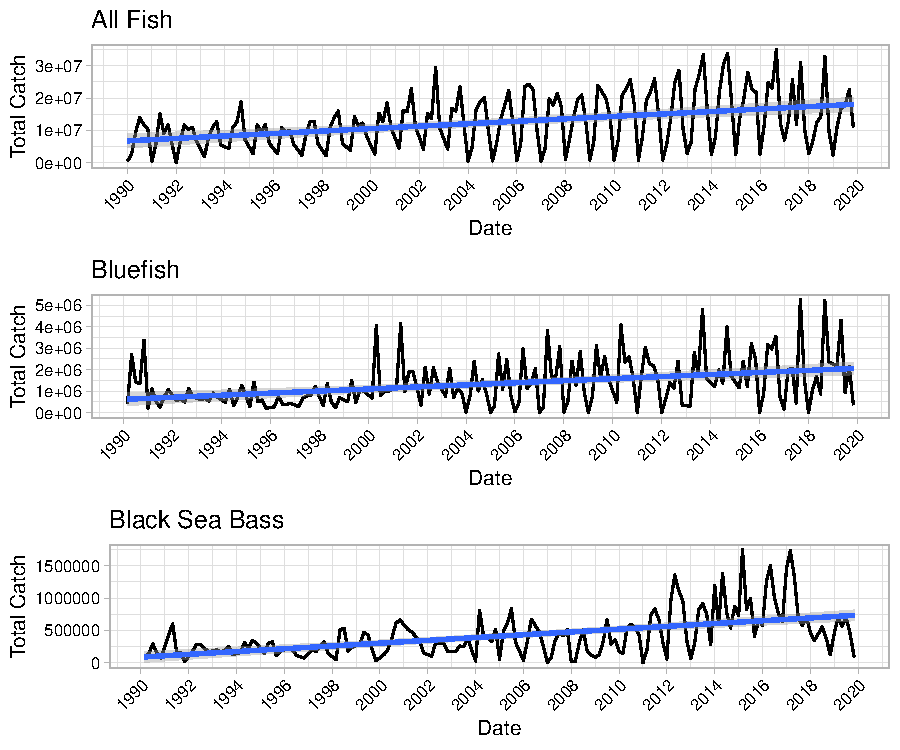
\includegraphics{Report_FishTrends_files/figure-latex/ggplot-1} 

\caption{Total Catch Patterns over Time}\label{fig:ggplot}
\end{figure}

\newpage

\hypertarget{analysis}{%
\section{Analysis}\label{analysis}}

\hypertarget{question-1-are-there-trends-in-the-amount-of-these-fish-caught-over-time-how-do-they-compare}{%
\subsection{Question 1: Are there trends in the amount of these fish
caught over time? How do they
compare?}\label{question-1-are-there-trends-in-the-amount-of-these-fish-caught-over-time-how-do-they-compare}}

\#\#Annie, certainly feel free to restructure these figures etc. as fits
with the text. I (Ardath) consolidated the p-values into a table to try
\& help make it visualize more clearly, too! I put the 3 tests into one
chunk, but/and we can rearrange \& smooth it out together on Sun, too.

\begin{quote}
\emph{Insert visualizations and text describing your main analyses.
Format your R chunks so that graphs are displayed but code and other
output is not displayed. Instead, describe the results of any
statistical tests in the main text (e.g., ``Variable x was significantly
different among y groups (ANOVA; df = 300, F = 5.55, p \textless{}
0.0001)''). Each paragraph, accompanied by one or more visualizations,
should describe the major findings and how they relate to the question
and hypotheses. Divide this section into subsections, one for each
research question.}
\end{quote}

\begin{quote}
\emph{Each figure should be accompanied by a caption, and each figure
should be referenced within the text}
\end{quote}

\begin{figure}[H]

\hfill{}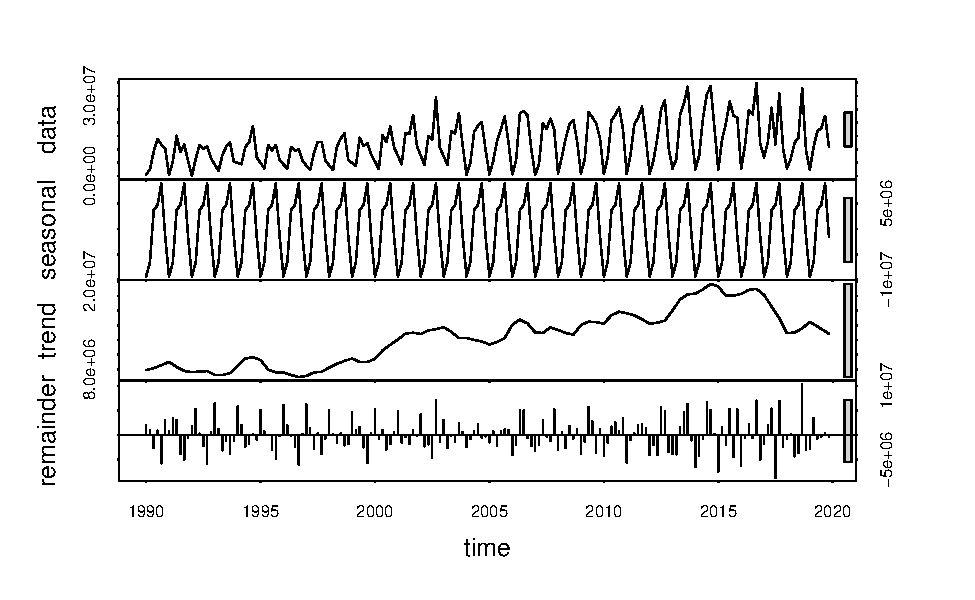
\includegraphics{Report_FishTrends_files/figure-latex/All Fish Trends-1} 

\caption{Seasonal and Trend Decomposition for All Fish Total Catch}\label{fig:All Fish Trends}
\end{figure}

\begin{figure}[H]

\hfill{}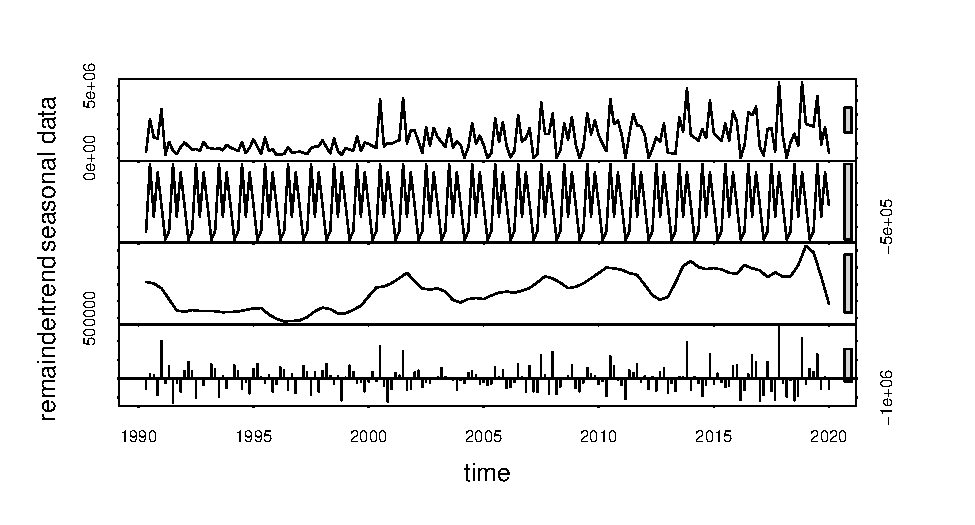
\includegraphics{Report_FishTrends_files/figure-latex/Bluefish Trends-1} 

\caption{Seasonal and Trend Decomposition for Bluefish Total Catch}\label{fig:Bluefish Trends}
\end{figure}

\begin{figure}[H]

\hfill{}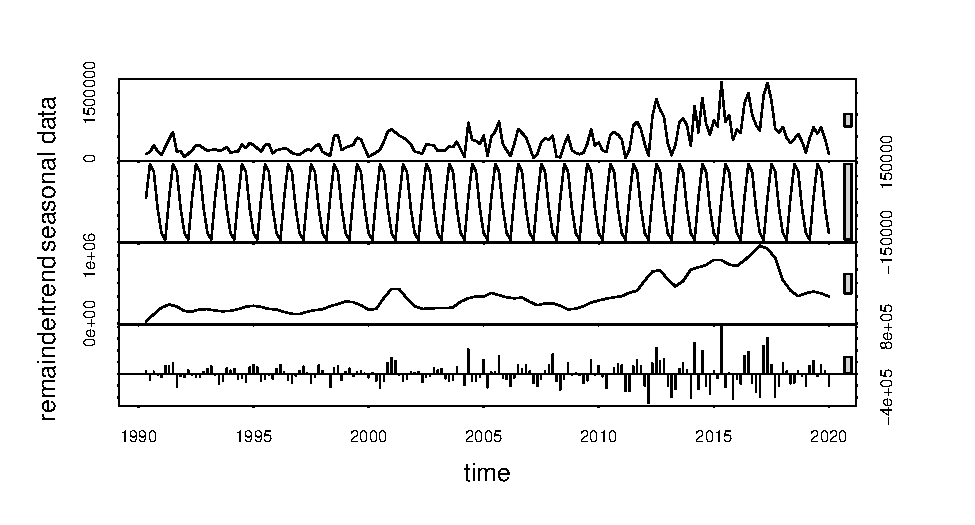
\includegraphics{Report_FishTrends_files/figure-latex/Black Sea Bass Trends-1} 

\caption{Seasonal and Trend Decomposition for Black Sea Bass Total Catch}\label{fig:Black Sea Bass Trends}
\end{figure}

\begin{table}[H]

\caption{\label{tab:table4}Seasonal Mann Kendall Tests}
\centering
\begin{tabular}[t]{l|r|l}
\hline
Fish Category & tau & 2-Sided P-value\\
\hline
All Fish & 0.4896552 & 0.000000e+00\\
\hline
Bluefish & 0.3235180 & 8.748902e-10\\
\hline
Black Sea Bass & 0.4095312 & 8.437695e-15\\
\hline
\end{tabular}
\end{table}

For both individual species and all species combined, \textbf{reject the
null hypothesis} that there is no trend.

\hypertarget{question-2-what-could-these-trends-look-like-in-the-future}{%
\subsection{Question 2: What could these trends look like in the
future?}\label{question-2-what-could-these-trends-look-like-in-the-future}}

\begin{flushright}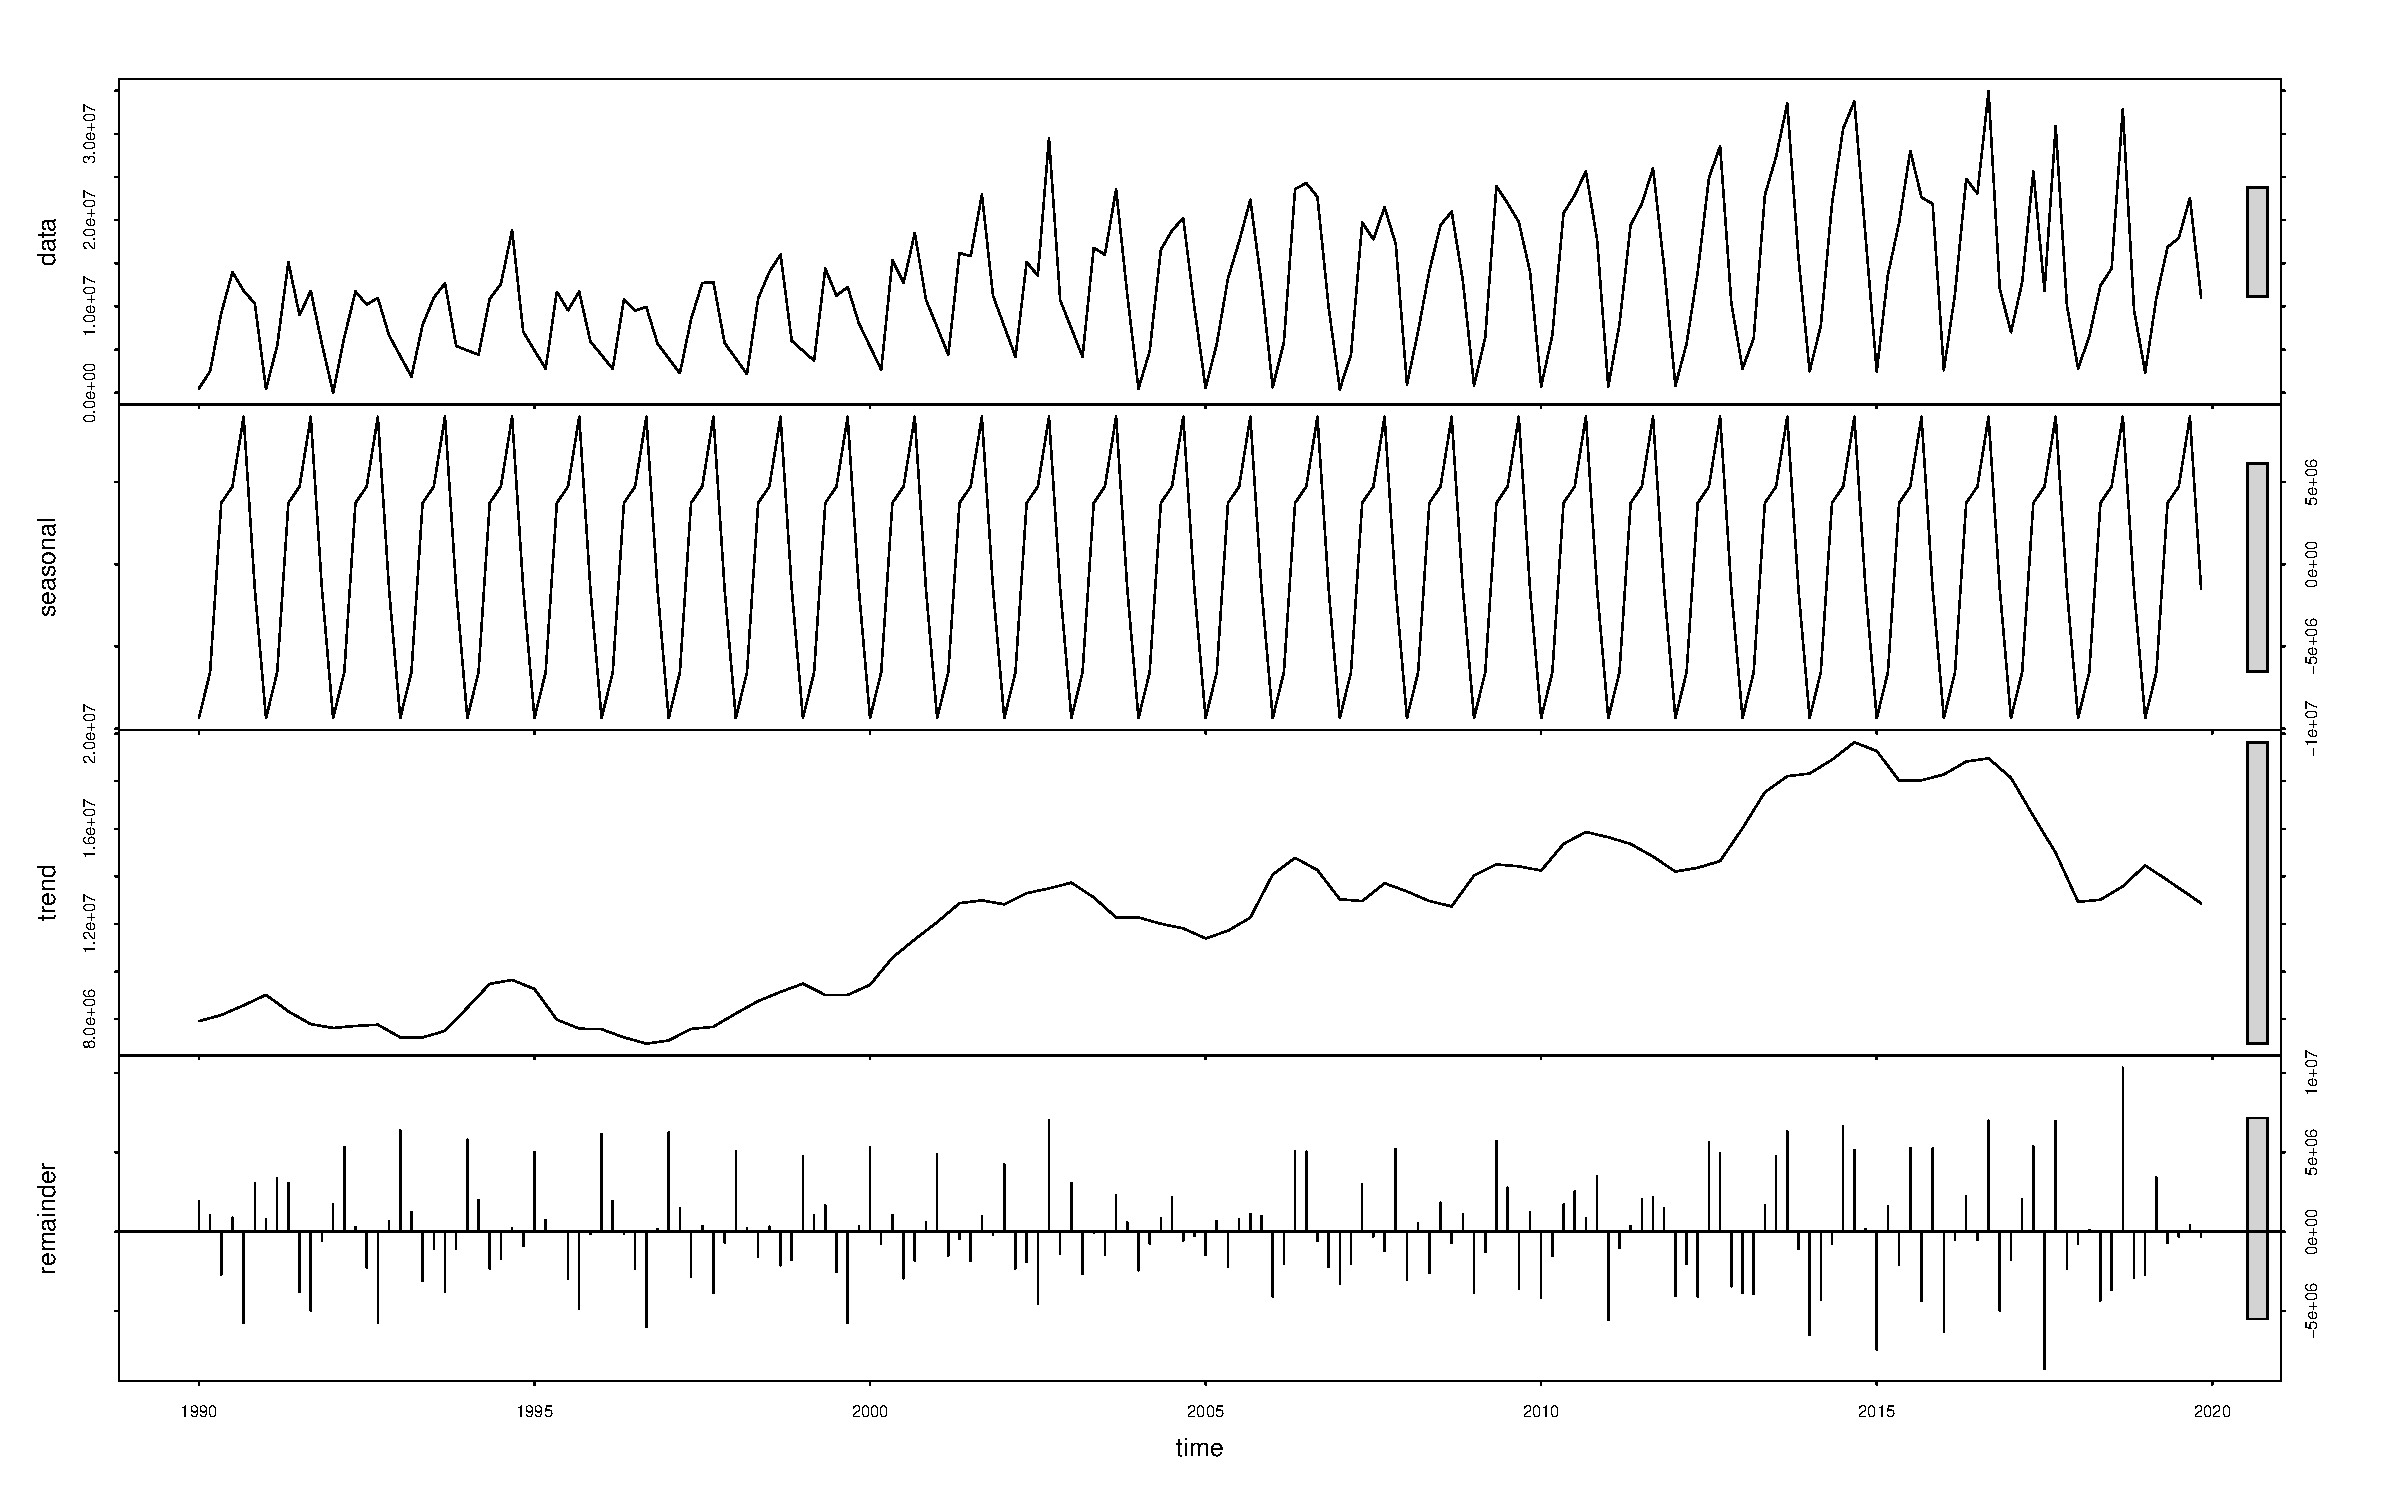
\includegraphics{Report_FishTrends_files/figure-latex/unnamed-chunk-1-1} \end{flushright}

\newpage

\hypertarget{summary-and-conclusions}{%
\section{Summary and Conclusions}\label{summary-and-conclusions}}

\begin{quote}
\emph{Summarize your major findings from your analyses in a few
paragraphs. What conclusions do you draw from your findings? Relate your
findings back to the original research questions and rationale.}
\end{quote}

\hypertarget{strong-seasonal-trends}{%
\subsection{Strong seasonal trends}\label{strong-seasonal-trends}}

NOAA marine recreational fishing catch totals for North Carolina show
strong seasonal trends. Many more fish are caught in the summer, and
much fewer fish are caught in the winter, as demonstrated above (Figure
1). The high seasonality for all three datasets analyzed was confirmed
with the Seasonal Mann Kendall Tests, where all three P-values
\textless{} 0.05 (Table 4).

This seasonality is likely influenced by recreational fishing patterns,
where fishers are more likely to fish in the warm summer weather than
the cool winter weather. Another potential cause for the seasonal trends
is fish abundance and migration patterns, with higher populations of
fish in North Carolina waters during the summer than during the winter.
Total catch trends for all fish and Black Sea Bass showed unimodal peaks
and valleys overall, while Bluefish showed bimodal trends (Figure 1).
These bimodal Bluefish peaks could be due to their seasonal migration
patterns (\href{http://www.asmfc.org/species/bluefish}{ASMFC 2021}).

\hypertarget{overall-positive-trend}{%
\subsection{Overall positive trend}\label{overall-positive-trend}}

\begin{itemize}
\tightlist
\item
  Increase in recreational fishing
\item
  Variation from changing regulations, behavior
\end{itemize}

\hypertarget{limitations}{%
\subsection{Limitations}\label{limitations}}

\begin{itemize}
\tightlist
\item
  Data collection: Estimates based on surveys of fishers
\item
  Interpolation
\item
  Uncertainty in forecasting
\end{itemize}

\hypertarget{future-recommendations}{%
\subsection{Future recommendations}\label{future-recommendations}}

\begin{itemize}
\tightlist
\item
  Comparisons of other species or other states
\item
  Catch per unit effort
\item
  Include earlier data
\end{itemize}

\newpage

\hypertarget{references}{%
\section{References}\label{references}}

\textless add references here if relevant, otherwise delete this
section\textgreater{}

\end{document}
